\documentclass{beamer}
\usepackage{beamerthemeshadow}
\usepackage{color}
%\usepackage[all]{xy}

%\newcommand{\comment}[1]{}
\newcommand{\comment}[1]{{\bf \tt  {#1}}}
\definecolor{ForestGreen}{RGB}{34,139,34}
\newcommand{\emcomment}[1]{\textcolor{ForestGreen}{\comment{Elena: {#1}}}}
\newcommand{\todo}[1]{\textcolor{blue}{\comment{To Do: {#1}}}}
\newcommand{\pscomment}[1]{\textcolor{red}{\comment{Paul: {#1}}}}
\newcommand{\mmcomment}[1]{\textcolor{magenta}{\comment{Max: {#1}}}}

\mode<presentation>
{
  \usetheme{Copenhagen} %%% Change later
 \usecolortheme{beaver}


  \setbeamercovered{transparent}
  % or whatever (possibly just delete it)
}
\setbeamertemplate{footline}[page number]{}


\begin{document}
\title{Developing a Graphical Library for a Clojure-based Introductory CS Course}
\author{Elena Machkasova, Paul Schliep, Max Magnuson}
\institute[UMM] % (optional, but mostly needed)
{
  Midwest Instruction and Computing Symposium
  
  University of Minnesota, Morris
}
\date{April 25, 2014}

\begin{frame}
  \titlepage
\end{frame}

\begin{frame}

  \frametitle{Outline}
\tableofcontents

\end{frame}

\section{Introduction to the project}

\begin{frame}
\frametitle{The Project}
\begin{itemize}
\item Contributing to an effort on adopting Clojure for an introductory course
\item Objective is to develop a graphical library for Clojure
\item We hope this graphical library can be useful for the introductory course
\end{itemize}
\end{frame}

\begin{frame}
\frametitle{Introduction to Clojure}
\begin{itemize}
\item Functional Programming Language in the Lisp family
\item Developed by Rich Hickey in 2007
\item Immutable Data Types and First Class Functions
\item Data Structures Such as Lists, Vectors, Hashmaps
\end{itemize}
\end{frame}

\begin{frame}[fragile]
\frametitle{Clojure Syntax}
\begin{itemize}
	\item Prefix Notation			
	\begin{verbatim}
		(<name of function> <argument 1> <argument 2> ...)
		(+ 2 2)
		-> 4
	\end{verbatim}
	\item Anonymous Functions
	\begin{verbatim}
		(fn [x] (* x x))
	\end{verbatim}
	\item Def
	\begin{verbatim}
		(def square-root[x] (* x x))
	\end{verbatim}
	\item First Class Functions
	\begin{verbatim}
		(map square-root [1 2 3 4])
		-> [1 4 9 16]
	\end{verbatim}
\end{itemize}
\end{frame}

\section{Goals and setup for an introductory course}

\begin{frame}
\frametitle{UMM's introductory CS course}
\begin{itemize}
\item Students are not expected to have prior programming knowledge
\item The course currently utilizes Racket to help teach key concepts
\item Racket is a functional language similar to Clojure
\item Functional languages help students learn concepts like recursion and higher order functions
\item The course makes use of Racket's graphical library 
\end{itemize}
\end{frame}

\begin{frame}
\frametitle{Introduction to functional approaches}
\begin{itemize}
\item Stylistic choice for programming
\item Immutable data types
\item Less dependency on order
\item First class functions
\end{itemize}
\end{frame}

\begin{frame}
\frametitle{Limitations of Clojure}
\begin{itemize}
\item Unintuitive error messages
\item Lacks a graphical library
\item Lack of an IDE suitable for beginner CS students
\end{itemize}
\end{frame}

\begin{frame}
\frametitle{Requirements for a graphical library}
\begin{itemize}
\item Reinforce functional approaches from Clojure
\item Implement Model-view-controller (MVC) similar to Racket's graphical library
\item Accessible to introductory students
\end{itemize}
\begin{center}
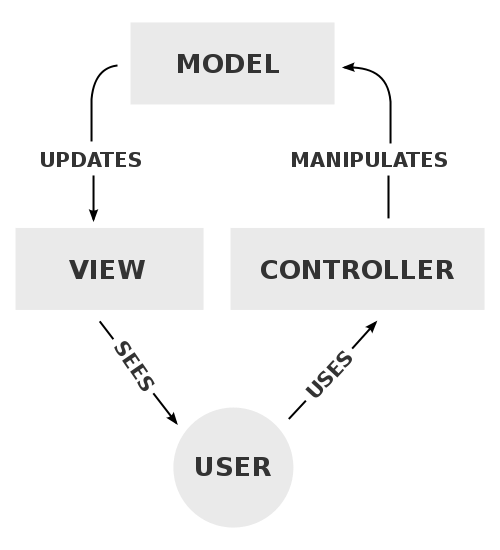
\includegraphics[width=100pt]{MVC-Process}
\end{center}
%\pscomment{Add graphic for MVC}
\end{frame}

\section{Developing a Clojure graphical library}

\begin{frame}
\frametitle{Overview of Quil}
\begin{itemize}
\item Open source graphical library for Clojure
\item Provides functionality suitable for introductory-level projects
\item Built on top of java swing
\item Continuously being developed
\end{itemize}
\end{frame}

\begin{frame}[fragile]
\frametitle{Developing programs with Quil}
\begin{itemize}
\item Defsketch
\item Works using frames and frame rate
\item Draws in layers
\item Supports input from keyboard and mouse
\begin{verbatim}
(defsketch example 
:title "Example"
:setup setup
:draw draw
:size [400 300])
\end{verbatim}
\end{itemize}
\end{frame}

\begin{frame}[fragile]
\frametitle{Example of a Quil program}
  \begin{columns}[T]
    \begin{column}{.5\textwidth}
      \begin{block}{Example Code:}
        \begin{verbatim}
(defn setup []
(frame-rate 1)
(background 200))

(defn draw []
(ellipse
(random (width))
(random (height))
100 100))
        \end{verbatim}
      \end{block}
    \end{column}

    \begin{column}{.5\textwidth}
      \begin{block}{Our Image}
        \begin{center}
        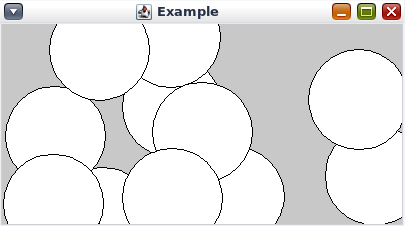
\includegraphics[width=150pt]{quil-example}
        \end{center}
      \end{block}
    \end{column}
  \end{columns}

\end{frame}

\begin{frame}
\frametitle{Issues with Quil}
\begin{itemize}
\item Imperative approaches
	\begin{itemize}
		\item Often requires direct manipulation of state
		\item Dependencies on order
		\item Inconsistent with introductory course goals
	\end{itemize}
\item Underdocumented API
\end{itemize}
\end{frame}

\section{Our graphical library}

\begin{frame}
\frametitle{Development of the graphical library}
\begin{itemize}
\item Abstracted over Quil's functions
	\begin{itemize}
	\item Defsketch
	\item Shapes
	\item Colors
	\item Text
	\end{itemize}
\item Handling state in a functional approach
\end{itemize}
\end{frame}


\begin{frame}
\frametitle{How our graphical library works}
\begin{itemize}
\item Separates handling of state
	\begin{itemize}
	\item MVC
	\item update
	\item display
	\end{itemize}
\item \todo{Something should go here, Max will remember what it is}
\end{itemize}
\end{frame}


\begin{frame}
\frametitle{Differences from Racket's graphical library}
\begin{columns}[T]
\begin{column}{.5\textwidth}
\begin{block}{Racket gives entire state to user}
\begin{center}
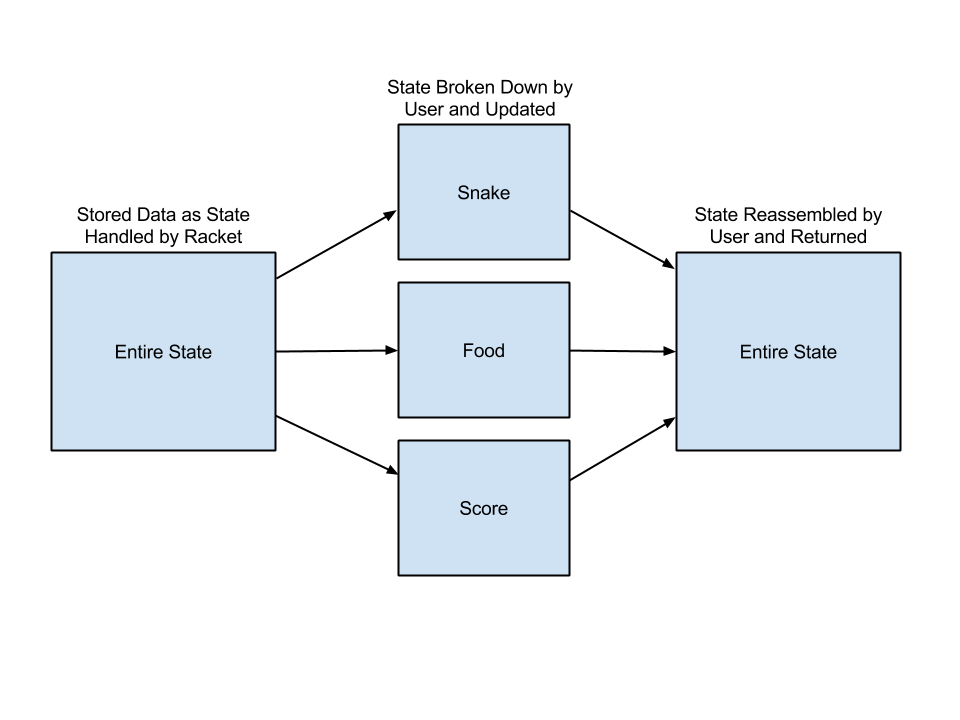
\includegraphics[width=150pt]{Rackets_State_Diagram}
\end{center}
\end{block}
\end{column}
\begin{column}{.5\textwidth}
\begin{block}{Our system breaks state down for the user}
\begin{center}
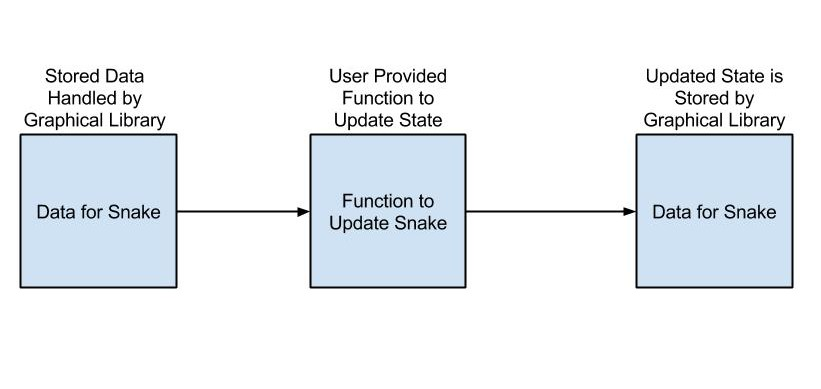
\includegraphics[width=150pt]{Handling_State_in_Graphical_Library}
\end{center}
\end{block}
\end{column}
\end{columns}
\end{frame}

\begin{frame} [fragile]
\frametitle{An example made using our graphical library}
\begin{verbatim}
(def states
{:snake [450 450 450 470 450 490 450 510] :snakeHeadX 450
:snakeHeadY 450 :foodX 150 :foodY 150 
:snake-direction "north"
:foodExists false :score 0})

(def updates
{:setup-drawing setup :update-snake update-snake})

(def display-order
[draw-snake draw-food redraw-canvas])
\end{verbatim}
%\todo{snake screenshot}
\end{frame}

\begin{frame}
\frametitle{Snake Example}
\begin{center}
\fbox{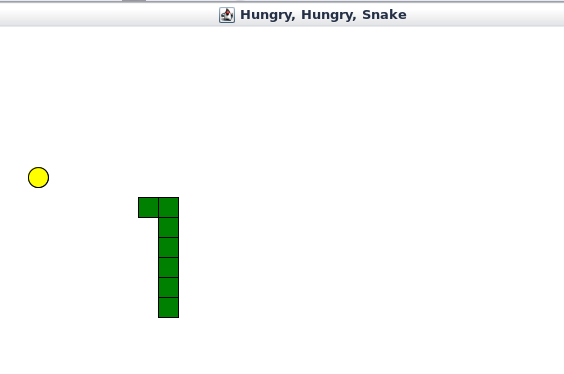
\includegraphics[width=200pt]{snake}}
\end{center}
\end{frame}


\section{Conclusions and Future Work}

\begin{frame}
\frametitle{Conclusions}
\begin{itemize}
\item Good start for abstracting over Quil's functions
\item More functional approach
\item Graphical library shows promise
\end{itemize}
\end{frame}

\begin{frame}
\frametitle{Future Work}
\begin{itemize}
\item Create our own macro to abstract over defsketch
\item Abstract over more functions in Quil
\item Develop an API with examples for students
\end{itemize}
\end{frame}

\begin{frame}
\frametitle{Acknowledgments and selected references}
Selected references:
\begin{itemize}
\item Quil https://github.com/quil/quil
\item Filleisen, M., Findler, R. B., Flatt, M. and Krishnamurthi, S. How to design programs: an introduction to programming and computing. MIT Press, Cambridge, MA, USA 2001.
\item Hickey, R. The clojure programming language. In Proceedings of the 2008 symposium on Dynamic languages(New York,NY,USA,2008),DLS'08,ACM,pp.1:1-1:1.
\end{itemize}
Acknowledgments:
The authors would like to thank...
\end{frame}


\end{document}
